\documentclass[12pt]{article}

%\usepackage[latin1]{inputenc}
\usepackage[utf8]{inputenc}
\usepackage{amsmath}
\usepackage{amsfonts}
\usepackage{amssymb}
\usepackage{graphicx}
\usepackage{multicol}
\usepackage{tabularx}
\usepackage{tikz}
\usetikzlibrary{arrows,shapes,automata,petri,positioning,calc}
\usepackage{hyperref}
\usepackage{tikz}
\usetikzlibrary{matrix,calc}
\usepackage{graphicx}
%\documentclass[journal,12pt,twocolumn]{IEEEtran}
\usepackage[none]{hyphenat}
\usepackage{listings}
\usepackage[english]{babel}

\usepackage{caption}
\usepackage[parfill]{parskip}
\usepackage{hyperref}
\usepackage{booktabs}
%\usepackage{setspace}\doublespacing\pagestyle{plain}
\def\inputGnumericTable{}
\usepackage{color}                                            %%
    \usepackage{array}                                            %%
    \usepackage{longtable}                                        %%
    \usepackage{calc}                                             %%
    \usepackage{multirow}                                         %%
    \usepackage{hhline}                                           %%
    \usepackage{ifthen}
\usepackage{array}
\usepackage{amsmath}   % for having text in math mode
\usepackage{parallel,enumitem}
\usepackage{listings}





    
\begin{document}
\title{\textbf{Straight Lines}}
\date{\vspace{-5ex}}
\maketitle

\section*{11$^{th}$ Maths - Chapter 10}
This is Problem-12 from Exercise 10.3

\begin{enumerate}
\item Two lines passing through point $\vec{A} = \begin{pmatrix} 2 \\ 3 \end{pmatrix}$ intersect each other at an angle of $60^\circ$. If the slope of one line is $2$, find the equation of the other line.
\end{enumerate}

\section{Solution}

Let $\vec{A} = \begin{pmatrix} 2 \\ 3 \end{pmatrix}$ be the given point, and the slope of one line $m_1 = 2$. Let the slope of the other line be $m$, and the angle between them be $60^\circ$.

\textbf{Input data:}
\begin{align*}
\text{Direction vector } \vec{m_1} &= \begin{pmatrix} 1 \\ 2 \end{pmatrix} \\
\text{Direction vector } \vec{m_2} &= \begin{pmatrix} 1 \\ m \end{pmatrix} \\
\cos \theta &= \frac{1}{2}
\end{align*}

The angle between two vectors is then expressed as:
\begin{align*}
\cos \theta &= \frac{\vec{m_1}^\top \vec{m_2}}{\|\vec{m_1}\|\|\vec{m_2}\|} \\
\frac{1}{2} &= \frac{\begin{pmatrix} 1 & 2 \end{pmatrix} \begin{pmatrix} 1 \\ m \end{pmatrix}}{\|\begin{pmatrix} 1 \\ 2 \end{pmatrix}\|\|\begin{pmatrix} 1 \\ m \end{pmatrix}\|} \\
\frac{1}{2} &= \frac{2m + 1}{\sqrt{5} \sqrt{m^2 + 1}} \\
\frac{1}{4} &= \frac{4m^2 + 4m + 1}{5m^2 + 5} \\
11m^2 + 16m - 1 &= 0
\end{align*}

From the quadratic equation, the roots can be found as:
\begin{align*}
m &= \frac{-b \pm \sqrt{b^2 - 4ac}}{2a} \\
m &= \frac{-16 \pm \sqrt{16^2 - 4(11)(-1)}}{2(11)} \\
m &= 0.06 \quad \text{or} \quad m = -1.514
\end{align*}

Therefore, the equation of the other line can be determined using these values.
\begin{enumerate}
\item Line passing through point $\vec{A} = \begin{pmatrix} 2 \\ 3 \end{pmatrix}$ with slope $m = 0.06$
\begin{align}
    \vec{n}^\top({\vec{x}-\vec{P}})&= 0 \\
    \vec{n} = \begin{pmatrix} m \\ -1 \end{pmatrix} \\
    \begin{pmatrix} 0.06 & -1 \end{pmatrix}(\vec{x}-\begin{pmatrix} 2 \\ 3 \end{pmatrix}) &= 0
\end{align}
then the eqation for m=0.06 is $y=0.06x+2.88$

\item Line passing through point $\vec{A} = \begin{pmatrix} 2 \\ 3 \end{pmatrix}$ with slope $m =-1.514$
\begin{align}
    \vec{n}^\top({\vec{x}-\vec{P}})&= 0 \\
    \vec{n} = \begin{pmatrix} m \\ -1 \end{pmatrix} \\
    \begin{pmatrix} -1.514 & -1 \end{pmatrix}(\vec{x}-\begin{pmatrix} 2 \\ 3 \end{pmatrix}) &= 0
\end{align}
Therefore then the equation is $1.514x+y=0.02$

 \begin{center}
 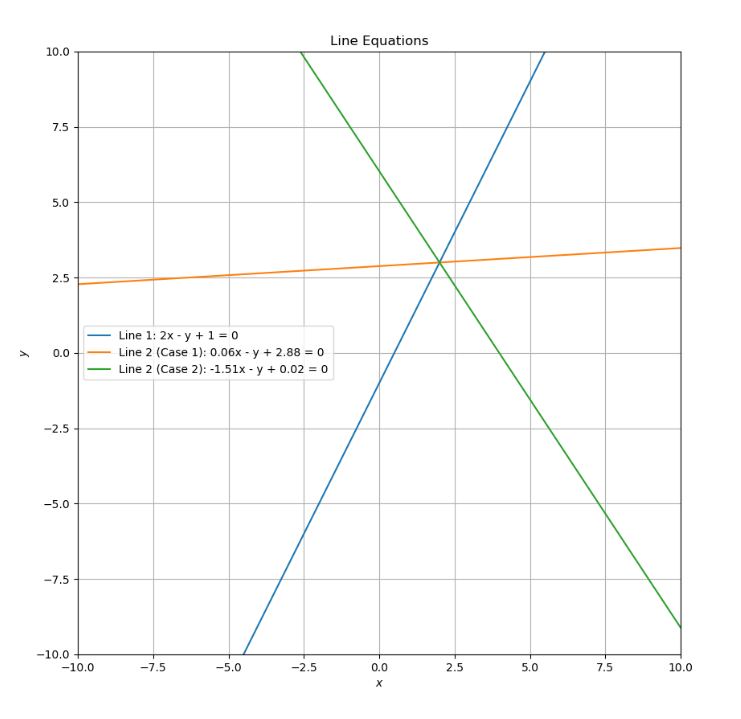
\includegraphics[width=\columnwidth]{line21.png}  
 \end{center}\vspace{1mm}
\end{enumerate}
\end{document}
